\documentclass[lmr,second,hyperref,rgb,hyperref,dvipsnames]{uom_thesis_casson}

%%%%% This is a generic preamble for article-like LaTeX documents. I can copy and paste this file into new documents to quickly make LaTeX styling which I like and is consistent with other documents I've typeset

\usepackage[a-3u]{pdfx}                 % PDF document properties
\usepackage{graphicx,psfrag}            % For postscript graphics files
    % \graphicspath{ {./images/} }
\usepackage{amsmath}                    % assumes amsmath package installed
    \allowdisplaybreaks[1]              % allow eqnarrays to break across pages
\usepackage{amssymb}                    % assumes amsmath package installed
\usepackage{url}                        % format hyperlinks correctly
\usepackage{rotating}                   % allow portrait figures and tables
\usepackage{multirow}                   % allows merging of rows in tables
\usepackage{lscape}                     % allows pages to be typeset in landscape mode
\usepackage{tabularx}                   % allows fixed width tables
\usepackage{verbatim}                   % enhanced version of built-in verbatim environment
\usepackage{footnote}                   % allows more control over footnote environments
\usepackage{float}                      % allows H option on floats to force here placement
\usepackage{booktabs}                   % improve table line spacing
\usepackage{lipsum}                     % for adding dummy text here
\usepackage[base]{babel}                % required for lisum package
\usepackage{subcaption}                 % for multiple sub-figures in a single float
\usepackage{siunitx}                    % add SI units
% \usepackage[dvipsnames]{xcolor}         % More colours
\usepackage{physics}
\usepackage{tabto}                      % \tab command
\usepackage{ragged2e}                   % Better ragged left
\usepackage{array}
\usepackage{caption}
\usepackage{mathtools}
\usepackage{bbm}
\usepackage{enumitem}
\usepackage{empheq}
\usepackage{gensymb}
\usepackage{textcomp}
\usepackage[bottom]{footmisc}           % Places footnotes at the bottom of the page
\usepackage{esvect}                     % For \vv
% \usepackage[a4paper, margin=1cm, tmargin = 1.5cm, bmargin=2cm, footskip = 1cm]{geometry}
\usepackage[skip = 10pt]{parskip}
\usepackage{indentfirst}                % I want my first paragraphs to always be indented
\usepackage{stackengine}
\usepackage{scalerel}
\usepackage{stmaryrd}
\usepackage{plimsoll}
% \usepackage{titlesec}
% \usepackage{MnSymbol}
\usepackage{accents}
\usepackage[super]{nth}
% \usepackage[T1,T2A]{fontenc}
% \usepackage[english, greek]{babel}
% \usepackage{textalpha}
\usepackage{unicode-math}  % Enter greek characters with unicode characters! α, β etc.
\usepackage{fancyhdr}




% \geometry{margin=1cm}
% \titlespacing*{\chapter}{0pt}{-40pt}{10pt}
\fancyfoot{}
\fancyfoot[LE,RO]{\thepage}

\newenvironment{boxequ}{\empheq[box=\widefbox]{equation}}{\endempheq}
\newenvironment{boxali}{\empheq[box=\widefbox]{align}   }{\endempheq}
\newenvironment{boxaliat}[1]{\empheq[box=\widefbox]{alignat=#1}}{\endempheq}

\newcommand*{\ndt}[1]{%
  \accentset{\mbox{\large\bfseries .}}{#1}}
\newcommand*{\nddt}[1]{%
  \accentset{\mbox{\large\bfseries .\hspace{-0.25ex}.}}{#1}}

% \usepackage{scalerel,stackengine}
% \stackMath
% \newcommand\widecheck[1]{%
% \savestack{\tmpbox}{\stretchto{%
%   \scaleto{%
%     \scalerel*[\widthof{\ensuremath{#1}}]{\kern-.6pt\bigwedge\kern-.6pt}%
%     {\rule[-\textheight/2]{1ex}{\textheight}}   %WIDTH-LIMITED BIG WEDGE
%   }{\textheight}% 
% }{0.5ex}}%
% \stackon[1pt]{\displaystyle #1}{\scalebox{-1}{\tmpbox}}%
% }
% \renewcommand\widehat[1]{%
% \savestack{\tmpbox}{\stretchto{%
%   \scaleto{%
%     \scalerel*[\widthof{\ensuremath{#1}}]{\kern-.6pt\bigvee\kern-.6pt}%
%     {\rule[-\textheight/2]{1ex}{\textheight}}   %WIDTH-LIMITED BIG HAT
%   }{\textheight}% 
% }{0.5ex}}%
% \stackon[1pt]{\displaystyle #1}{\scalebox{-1}{\tmpbox}}%
% }

\newcommand{\sus}[1]{$^{\mbox{\scriptsize #1}}$}
\newcommand{\sub}[1]{$_{\mbox{\scriptsize #1}}$}
\newcommand{\chap}[1]{Chapter~\ref{#1}}
\newcommand{\sect}[1]{Section~\ref{#1}}
\newcommand{\fig}[1]{Fig.~\ref{#1}}
\newcommand{\tabl}[1]{Table~\ref{#1}}
\newcommand{\equ}[1]{(\ref{#1})}
\newcommand{\appx}[1]{Appendix~\ref{#1}}

\newcommand{\blue}[1]{\colorlet{saved-blue}{.}\color{NavyBlue}#1\color{saved-blue}}
\newcommand{\red}[1]{\colorlet{saved-red}{.}\color{Red}#1\color{saved-red}}
\newcommand{\green}[1]{\colorlet{saved-green}{.}\color{PineGreen}#1\color{saved-green}}
\newcommand{\purple}[1]{\colorlet{saved-purple}{.}\color{Plum}#1\color{saved-purple}}
\newcommand{\orange}[1]{\colorlet{saved-orange}{.}\color{YellowOrange}#1\color{saved-orange}}
\newcommand{\brown}[1]{\colorlet{saved-brown}{.}\color{Brown}#1\color{saved-brown}}
\newcommand{\pink}[1]{\colorlet{saved-pink}{.}\color{CarnationPink}#1\color{saved-pink}}


% \renewcommand{α}{\alpha}
% \renewcommand{β}{\beta}
% \newcommand{γ}{\gamma}
% \renewcommand{δ}{\delta}
% \newcommand{\e}{\epsilon}
% \newcommand{\z}{\zeta}
% \renewcommand{\th}{\theta}
% \renewcommand{\i}{\iota}
% \renewcommand{\k}{\kappa}
% \renewcommand{λ}{\lambda}
% \renewcommand{ρ}{\rho}
% \renewcommand{\t}{\tau}
% \newcommand{\s}{\sigma}
% \renewcommand{\u}{\upsilon}
% \renewcommand{ρ}{\rho}
% \newcommand{\vr}{\varrho}
% \newcommand{ω}{\omega}
% \newcommand{\f}{\varphi}
% \renewcommand{Λ}{\Lambda}
% \newcommand{\G}{\Gamma}
% \newcommand{Δ}{\Delta}
% \newcommand{\Th}{\Theta}
% \newcommand{Ω}{\Omega}

\newcommand{\fa}{\forall\:}
\newcommand{\fe}{\exists\:}

\renewcommand{\rm}{\mathrm}
\newcommand{\bb}[1]{\mathbb{#1}}
\newcommand{\cl}[1]{\mathcal{#1}}
\newcommand{\fk}[1]{\mathfrak{#1}}

\newcommand{\Le}{\rm{Le}}
\renewcommand{\Pr}{\rm{Pr}}
\newcommand{\Ma}{\rm{Ma}}
\newcommand{\Ze}{\rm{Ze}}
\newcommand{\Mk}{\cl{M}}
\newcommand{\Fr}{\rm{Fr}}
\newcommand{\Pe}{\rm{Pe}}
\newcommand{\Da}{\rm{Da}}
\newcommand{\Ka}{\rm{Ka}}
% \renewcommand{\Re}{\rm{Re}}
% \newcommand{\Im}{\rm{Im}}
\newcommand{\rhs}{\rm{RHS}}

\renewcommand{\vb}[1]{\symbf{#1}}
\def\stacktype{S}
\newcommand{\hvec}[1]{\stackon[-0.5pt]{#1}{\scaleobj{0.9}{\rightharpoonup}}}
% \newcommand{\nhat}[1]{\stackon[-3.5pt]{#1}{\scaleobj{0.9}{\textasciicircum}}}
\newcommand{\nhat}[1]{\widehat{#1}}
\newcommand{\uvec}[1]{\nhat{\vb{#1}}}
\newcommand{\ftvar}[1]{\stackon[0.5pt]{#1}{\scaleobj{0.75}{\sim}}}
\newcommand{\vvt}[1]{\vv{\vv{#1}}}
\newcommand{\und}[1]{\underline{#1}}
\newcommand{\undt}[1]{\und{\und{#1}}}

\newcommand{\ft}{\cl{F}}
\newcommand{\ift}{\cl{F}^{-1}}
\DeclareMathOperator{\DFT}{DFT}
\DeclareMathOperator{\IDFT}{IDFT}

\newcommand{\angs}[1]{\left\langle #1 \right\rangle}
\newcommand{\ceil}[1]{\left\lceil #1 \right\rceil}
\newcommand{\floor}[1]{\left\lfloor #1 \right\rfloor}
\newcommand{\bbra}[1]{\left\llbracket \mspace{2mu} #1 \mspace{2mu} \right\rrbracket}
\newcommand{\aang}[1]{\left\llangle #1 \right\rrangle}
% \newcommand{\ccor}[1]{\ullcorner #1 \ulrcorner}
\newcommand{\ccor}[1]{\boldsymbol{\ullcorner} #1 \boldsymbol{\ulrcorner}}

\renewcommand{\dim}{N_{\rm{D}}}

\newcommand{\mDv}[1]{\frac{\mathrm{D}}{\mathrm{D} #1}}
\newcommand{\mdv}[2]{\frac{\mathrm{D} #1}{\mathrm{D} #2}}
\newcommand{\gbar}{\barγ}

\newcommand{\tang}{\parallel}



\captionsetup{width=\textwidth} 

\newcommand*\widefbox[1]{\fbox{\hspace{1.5mm}#1\hspace{1.5mm}}}
\setlength\fboxsep{3mm}


% Note backref=true adds a page number (and hyperlink) to each reference so you can easily go back from the references to the main document. You may prefer backref=false if you need to stick strictly to a given reference style
\usepackage[style = ieee, backend = biber, backref = true, hyperref = auto]{biblatex}
\renewcommand*{\bibfont}{\small}
\DefineBibliographyStrings{english}{backrefpage = {cited on p\adddot},  backrefpages = {cited on pp\adddot}}


\addbibresource{references.bib}



\begin{document}


\makeatletter
\title{\xmp@Title}
\author{\xmp@Author}
\makeatother

\faculty{Science and Engineering}
\department{School of Engineering}
\submitdate{2025, Autumn}
%\wordcount{}
\maketitle


\begin{abstract}

In this report, we tackle the problem of expensive thermoacoustic simulations by introducing a new boundary conditions (BCs) scheme based off the Navier-Stokes characteristic BCs (NSCBCs) formulation. This truncates a flame tube by restricting DNS to the flame and its surrounding hydrodynamics and allows tube acoustics to be modelled using a simple delay on acoustics leaving this DNS domain. Code schematics for this method, dubbed the acoustic delay characteristic BCs (ADCBCs), are presented as they relate to implementation into the NSCBC scheme. Instabilities resulting from the acoustic-DNS coupling can be reduced by increased tangential filtering at the boundaries, although this is unlikely to be an issue when one-dimensional approximations are made at each boundary node. Simulations are then performed using these boundary conditions and show that solutions show excellent agreement with the acoustic eigenmodes of a one-dimensional flame tube system with no damping elements. Comparisons are drawn between ADCBCs and the existing delayed time-domain impedance BCs (D-TDIBC) which instead models the expected acoustic impedance at the truncated boundary according to the acoustic delay observed. Various benefits of the method include: the massive increase to computational cost as only one part of the tube is discretised; the delay times can trivially change allowing the flame region to be translated along the tube's length; ADCBCs are implemented as an additional layer on top of NSCBCs with few additional requirements being made, allowing parts of the NSCBCs to be modularly reintroduced; only a simple one-dimensional linear model for acoustics is currently being used, although other nonlinear or higher-dimensional models could be used; similar modelling could be done to model non-trivial upstream and downstream tube end impedances.

\end{abstract}


\uomtoc


\uomstartmainbody % Don't delete. used to flag to the hyperlinks in the PDF that the main content is starting


\chapter{Literature Review} \label{ch:lit-review}
\section{Prior Markstein Number Methods}

Finding the Markstein number is crucial to predicting the behaviour of flames.

LITERATURE:
\begin{itemize}
\item \cite{clavin1982EffectsMolecularDiffusion} the first theoretical prediction of Markstein number from asymptotic theory
\item \cite{matalon1982FlamesGasdynamicDiscontinuities} also predicted the same Markstein number in the same year from similar asymptotics
\item \cite{searby1991ParametricAcousticInstability} proposes Mathieu model for secondary thermoacoustic instability. This is used to predict Markstein numbers experimentally by comparing sound frequency at the onset of parametric instability to the acoustic amplitude and comparing this data to theoretical predictions at different Markstein numbers. The disturbance wavenumber is also proposed as a method to find this Markstein number in a similar way.
\item \cite{delfin2024DeterminationMethodMarkstein} measures Markstein numbers using the proposed method from \cite{searby1991ParametricAcousticInstability} by measuring disturbance wavenumbers at the onset of secondary instability and comparing them to theoretical values.
\item \cite{day2009TurbulenceEffectsCellular} calculates Markstein numbers from simulation data for lean premixed H2-air combustion by computing JPDFs of flame speed against flame curvature. Each data point in these JPDFs is an \emph{integral tubes} (the area bounded by 3 or more integral curves, in 3D) of $\vec{\nabla} c$ for $c$ the reactant progress variable with values taken at $c=0.98$, representing the position of the flame.
\item \cite{howarth2022EmpiricalCharacteristicScaling} and \cite{howarth2023ThermodiffusivelyunstableLeanPremixed} follow the same method as \cite{day2009TurbulenceEffectsCellular}, but incorporates the strain term to the right-hand side calculation, uses $c=0.9$. Care is taken to ensure that the chosen flame surface is representative of the flame. They also evaluate individual Markstein numbers for the curvature and strain term on the RHS, as suggested in \cite{clavin2011CurvedStretchedFlames} (TALK ABOUT THIS PAPER ABOVE??).
\item \cite{davis2002MarksteinNumbersCounterflow} compares markstein numbers calculated from unburnt and burnt velocity values. (NEED TO READ??)
\item Al Sarraf ??
\item Aldredge ??
\end{itemize}




\section{Direct Numerical Simulation}

\cite{orszag1970AnalyticalTheoriesTurbulence, domingo2023RecentDevelopmentsDNS, chen2011PetascaleDirectNumerical, yang2015LargeeddySimulationPresent, veynante2002TurbulentCombustionModeling, moin1998DirectNumericalSimulation, tennekes1972FirstCourseTurbulence}

% The most blunt way to simulate a fluid system would be one where you try to accurately simulate every detail involved in the fluid.
% This idea was first studied by Orszag, where he defines direct numerical simulations as a numerical simulation with enough grid points to full resolve the smallest physical phenomena in the system
% Originally, Orszag studied this in the context of turbulent flows. In turbulent flows, we have vortices not only on the order of the typical flow length scale $L$, called the integral length scale, but also of sizes all the way down to the smallest turbulence scale known as the kolmogorov microscale, where the rate at which viscous dissipation effects dampen vortices far exceeds the inertial forces of the vortex.
% The size of this kolmogorov length scale is determined by the turbulent reynolds number and the integral scale with the relationship

% An alternative method that is widely used is LES and involves using models to estimate the transfer of energy at the smallest scale rather than fully simulating them [cite les review: Yang 2015]
% DNS for turbulent combustion are reviewed in \textbf{Domingo and Vervisch 2023} (with connection to LES) and \textbf{Chen 2011}.

% For small-scale, low-speed methan-air and hydrogen-air combustion, the flows we look at have similar properties to air, so are not very viscous meaning the smallest scale vortices in a fully developed turbulent may be ~...?
% But the turbulence usually isn't our biggest worry, since we also have the thin region that the reaction is taking place to resolve, usually only 300 {\textmu}m which is resolved with ~15 nodes in a high order code
% Regardless, when performing DNS careful consideration must be made to use ample sample points

% ?? DNS with simple transport / chemical schemes?




\section{Characteristic Boundary Conditions}

\cite{thompson1987TimeDependentBoundary, thompson1990TimeDependentBoundaryConditions, poinsot1992BoundaryConditionsDirect, poinsot2005TheoreticalNumericalCombustion, sutherland2003ImprovedBoundaryConditions}

% [Thompson 1987, 1990, Poinsot and Lele 1992, Sutherland and Kennedy 2003, Poinsot and Veynante 2005]


% Many types of boundary conditions may be chosen for combustion schemes:
%% Periodic are very simple to enforce numerically so require no elaboration
%% No-slip or slip wall conditions
%% isothermal or adiabatic walls
%% acoustically reflecting or non-reflecting walls or inflow / outflow
%% In the case of inflow / outflow many more cases

% In most of these cases, we can use the formalism called characteristic boundary conditions (characteristic BCs)




% The simplest boundary conditions, i.e. those with constant (Dirichlet) boundary values (p=const), usually reflect acoustic waves back toward the interior of the domain. For most situations we want to simulate, this doesn't represent the physical situation, where we would rather pretend the medium continues outside of the compuational domain. This motivates a need for boundary conditions which do not reflect acoustic waves - non-reflecting boundary conditions. The formalisms are based of characteristic waves entering / leaving the domain

% Fixed velocity inlets give full reflections, so cannot be used in a non-reflecting case.

% Immersed boundary methods are also an option and open up possibilities for boundaries not restricted specific node placement, especially for moving boundaries. But as detailed in King 2022, these a largely restricted to lower order accuracy at these boundaries (cite, and for what reason?).







\section{Mesh-free Methods}

\cite{monaghan1992SmoothedParticleHydrodynamics, vacondio2021GrandChallengesSmoothed}






\section{Thermoacoustic Combustion Instabilities}

% Thermoacoustics background - can cover what was in 1YR



\chapter{The `Sunset-Flames' Combustion Software} \label{ch:sunset}


\section{LABFM}

\cite{king2024MeshFreeFrameworkHighOrder, king2020HighOrderDifference, king2024MeshfreeFrameworkHighorder, king2022HighorderSimulationsIsothermal, king2024SunsetFlamesDNSCode}


\subsection{High-Order Interpolations}

% in keeping with other methods, where interpolation is the first step to gradient approximations

Before considering gradient approximations, we first consider interpolations, hoping that they are simpler and elucidate a method for us. We consider a location $\vec{x}$ surrounded locally by finitely many nodes $\vec{x}_j \in \cl{S}(\vec{x})$ which are enumerated by $j \in \cl{N}(\vec{x})$, where $\abs{\vec{x} - \vec{x}_j} < h(\vec{x})$ and a function $\phi = \phi(\vec{x})$ which is \emph{smooth enough}.\footnote{Some elaboration.} Then we express the interpolated value $\phi(\vec{x})$ as a linear combination of the surrounding function values $\phi_j = \phi(\vec{x}_j)$:
\begin{equation} \label{eqn:L}
L^{\rm{int}}[\phi](\vec{x}) \equiv \sum_{j \in \cl{N}(\vec{x})} \phi_j w^{\rm{int}}(\vec{x}, \vec{x}_j) \approx \phi(\vec{x}).
\end{equation}
To find the weights $w^{\rm{int}}(\vec{x}, \vec{x}_j)$, we must observe the contribution of function derivatives into $\phi$ by means on Taylor series. This derivative space is expressed as projections of the vectors of derivatives of $\phi$:
\begin{equation}
\vv{D}[\phi] = \left(1, \pdv{\phi}{x}, \pdv{\phi}{x}, \pdv[2]{\phi}{x}, \pdv[2]{\phi}{x}{y}, \pdv[2]{\phi}{x}, \dots \right)^T
\quad \text{and} \quad
\vv{D}_k[\phi] = \left(1, \pdv{\phi}{x}, \pdv{\phi}{x}, \dots, \pdv[k]{\phi}{x}, \dots, \pdv[k]{\phi}{y} \right)^T,
\end{equation}
where we have assumed that $\phi$ is a scalar field over two spatial dimensions $\vec{x}=(x, y)$, although the method may be simply extended to any number of dimensions. In this notation, interpolation is just $\phi(\vec{x}) = \vv{D}[\phi](\vec{x}) \cdot \vv{C}^{\rm{int}} = \vv{D}_k[\phi](\vec{x}) \cdot \vv{C}_k^{\rm{int}}$ where $\vv{C}^{\rm{int}} = (1, 0, 0, 0, 0, 0, \dots)^T$ and $\vv{C}_k^{\rm{int}} = (1, 0, 0, \dots, 0,)^T$, which is of the same length as $\vv{D}_k$. Then, upon introducing vectors of monomials:
\begin{equation}
\vv{X}(\vec{x}) = \left(1, x, y, \frac{1}{2!} x^2, xy, \frac{1}{2!} y^2, \dots \right)^T
\quad \text{and} \quad
\vv{X}_k(\vec{x}) = \left(1, x, y, \dots, \frac{1}{k!} x^k, \dots, \frac{1}{k!} y^k \right)^T,
\end{equation}
we can simplify down the Taylor expansion of $\phi$ around the point $\vec{x}$ for any $\vec{x}_j$ as:
\begin{subequations}
\begin{align}
\phi_j &= \phi(\vec{x}) + \pdv{\phi}{x}\bigg|_{\vec{x}} (x_j - x) + \pdv{\phi}{y} \bigg|_{\vec{x}} (y_j - y)  \\
& \qquad  \quad \ \, + \frac{1}{2!} \pdv[2]{\phi}{x}\bigg|_{\vec{x}} (x_j - x)^2 + \pdv[2]{\phi}{x}{y}\bigg|_{\vec{x}} (x_j - x) (y_j - y) + \frac{1}{2!} \pdv[2]{\phi}{y}\bigg|_{\vec{x}} (y_j - y)^2 + \dots \\
&= \vv{D}[\phi](\vec{x}) \cdot \vv{X} (\vec{x}_j - \vec{x}),
\end{align}
\end{subequations}
which may be truncated to $\phi_j \approx \vv{D}_k[\phi](\vec{x}) \cdot \vv{X}_k (\vec{x}_j - \vec{x})$ with $\cl{O}(h^{k + 1})$ truncation error. Rewriting \equ{eqn:L} in this formulation:
\begin{subequations}
\begin{align}
L^{\rm{int}}[\phi](\vec{x}) &= \vv{D}[\phi](\vec{x}) \, \cdot \sum_{j \in \cl{N}(\vec{x})} \vv{X} (\vec{x}_j - \vec{x}) w^{\rm{int}}(\vec{x}, \vec{x}_j) \\
&\approx \vv{D}_k[\phi](\vec{x}) \, \cdot \sum_{j \in \cl{N}(\vec{x})} \vv{X}_k (\vec{x}_j - \vec{x}) w^{\rm{int}}(\vec{x}, \vec{x}_j) \equiv \vv{D}_k[\phi](\vec{x}) \cdot \vv{B}_k^\rm{int}(\vec{x}) \\
&\approx \vv{D}_k[\phi](\vec{x}) \cdot \vv{C}_k^{\rm{int}}
\end{align}
\end{subequations}
So our problem now involves finding the correct values of $w^{\rm{int}}(\vec{x}, \vec{x}_j)$ such that the \emph{vector of moments} $\vv{B}_k^{\rm{int}}(\vec{x})$ of $w^{\rm{int}}$ approximates $\vv{C}_k^\rm{int}$. For consistency then, we require that the first component is independent of $h$:
\begin{equation}
1 = C_k^{\rm{int}, 0} \approx B_k^{\rm{int}, 0}(\vec{x}) = \sum_{j \in \cl{N}(\vec{x})} w^{\rm{int}} (\vec{x}, \vec{x}_j),
\end{equation}
so $w^{\rm{int}} = \cl{O}(h^0)$, where the superscript zeroes represent the leading vector component. The resulting error in this approximation is $\cl{O}(h^{k + 1})$, coming from the combined error from truncating the Taylor expansion of $\phi_j$ and approximating $w^{\rm{int}}$.

What's left is to find the weights of $w^{\rm{int}}$ in a way which can be solved for at any point $\vec{x}$ surrounded by nodes $\vec{x}_j$. To do this, we separate $w^{\rm{int}}$ into some anisotropic dependence of $\vec{x}$ on the surrounding nodes from the contribution that the action of interpolation has. This is done by writing it as the weighted sum of some anisotropic basis functions:
\begin{equation}
w^{\rm{int}}(\vec{x}, \vec{x}_j) = \vv{W}_k(\vec{x}_j - \vec{x}) \cdot \vv{\Psi}_k^{\rm{int}}(\vec{x})
\end{equation}
where the anisotropy is seen in the dependence of $\vv{W}_k$ on $(\vec{x}_j - \vec{x})$, which includes directional information, rather than $|\vec{x}_j - \vec{x}|$ (contrasting to the radial basis function method). Assuming that $\vv{W}_k$ comprises some known \emph{anisotropic basis functions} (ABFs) [we can find them according to king 2022], we must find the vector of weights $\vv{\Psi}_k^{\rm{int}}(\vec{x})$. This is done by substituting the new form into the vector of moments:
\begin{align}
\vv{C}_k^\rm{int}
\approx \vv{B}_k^{\rm{int}}(\vec{x})
= \left( \sum_{j \in \cl{N}(\vec{x})} \vv{X}_k (\vec{x}_j - \vec{x}) \otimes \vv{W}_k(\vec{x}_j - \vec{x}) \right) \cdot \vv{\Psi}_k^{\rm{int}}(\vec{x})
\equiv M(\vec{x}) \cdot \vv{\Psi}_k^{\rm{int}}(\vec{x})
\end{align}
where $M$ is a $n \times n$ matrix and $n$ is the number of components of $\vv{C}_k^\rm{int}$. The vector of weights $\vv{\Psi}_k^{\rm{int}}(\vec{x})$ is found when the linear system is solved. Carrying over the error terms from previous steps, we expect convergence on the order $\cl{O}(h^{k + 1})$.

% we require a number of nodes to ensure the linear system has a solution. typically the kernel is non-trivial, so we just need one solution
% The number of nodes required per stencil ~70 in 2D makes it expensive to calculate the weights for a given position to interpolate to. If you know beforehand where to interpolate to, this becomes cheap as it is done in preprocessing

% Cannot yet show convergence information unless I code this stuff myself (which I don't want to do)

% Stability?

% M condition number???? (worth mentioning but not extensively)


\subsection{High-Order Derivatives}

% Like other methods, we may wish to use this method of interpolation to find gradients as well. For classical methods, this is essentially done by differentiating the formulae we have already found. For LABFM, we have the benefit of a formulation where we can simply search for solutions where C = (0, 1, 0, ..) 
% For use in PDEs, we want gradients at points we have phi_i information at, so x becomes one of the nodes
% Since we are looking for derivatives now, we no longer require information on the absolute value phi_j, but the scalar relative to its value at the centre, phi_ji. The only change to the analysis above is that vectors e.g. X = (1, x, x^2/2, ...) -> X = (x, x^2/2) since the value phi_i = D[phi](x_i)^0 X(x_j - x_i)^0 is not needed
% Show new 'formula' and write in discrete notation X_ji not X(x_j - x_i)

% Ending - COST: we can do this process in any number of dimensions, although the cost scales rapidly from 2D to 3D as many more nodes x_j are contained within stencils. Usually have 70-80 nodes per stencil in 2D, making it quite expensive
% good part is that finer geometries are easy to resolve by scattering nodes. Mention how boundaries are discretised with 5 layers of nodes for upwinded finite differencing for outgoing waves
% Lagrangian methods are hard as above





% \blue{

% $$f(x) = y,\quad \text{also}, \quad \overset{\rightsquigarrow}{C}$$

% How do mesh-free methods help us generally, and what does LABFM do which is especially helpful? Mesh-free methods generally:
% \begin{itemize}
% \item FEM famously requires meshing which needs to be of high quality, such that a significant portion of the total man-hours are spent actually creating a high-quality mesh. Mesh free methods almost entirely avoid this (the node set still needs to be of high quality though.)
% \item Mesh free methods are much more suitable to Lagrangian methods, where nodes can move with the simulation. This works well with incompressible and free-surface flows
% \item Node sets for complex geometries are relatively easy to produce, where finite difference methods are not an option and FEM is difficult to make a node set for (kind of the first point)
% \end{itemize}

% and LABFM specifically:
% \begin{itemize}
% \item 
% \end{itemize}

% why do we use *anisotropic* basis functions rather than the isotropic ones we may use for sph (is this true?)? we want a general difference operator, which takes nodes unevenly located rotationally so we need to make up for this rotational asymmetry by including it also in our basis functions.

% }



\section{Navier-Stokes Characteristic Boundary Conditions (NSCBC)}

% Include diffusive effects



\subsection{Locally One-Dimensional Inviscid (LODI)}

% Cite Thompson 1987, 1990, 1987 lectures?

Any hyperbolic system can be written in the form:
\begin{equation} \label{eqn:hyp-source}
\pdv{\und{U}}{t} + \vec{\nabla}\cdot\und{\vec{F}} + \und{B} = 0,
\end{equation}
where $\und{U}$ are the $N_\rm{V}$ conservative variables, $\und{\vec{F}}$ are the fluxes for each of these variables in each dimension and $\und{B}$ are source terms. Since we do not include diffusion effects, we assume that these terms are non-diffusive. % Also explain notation -> space in bold, variables underlined, matrices double underlined
This equation is unique up to linear combinations of the conserved variables, but can be transformed into a form for the primitive variables $\und{u}$, from which the characteristics will arise:
\begin{equation}
\pdv{\und{u}}{t} + \undt{\vec{A}} \cdot \vec{\nabla} \und{u} + \und{b} = 0
\end{equation}
where
\begin{equation}
P_{ij} \equiv \pdv{U_i}{u_j},
\quad
\vec{\Phi}_{ij} \equiv \pdv{\vec{F}_i}{u_j},
\quad
\undt{\vec{A}} \equiv \undt{J}^{-1}\undt{\vec{\Phi}}
\quad \text{and} \quad
\und{b} \equiv \undt{{P}}^{-1}\und{B}.
\end{equation}
The matrix $\undt{P}$ is the Jacobian matrix, $\undt{\vec{A}}$ represents the convection of the variables due to the other variables and themselves (e.g. $(\vec{u} \cdot \vec{\nabla})\vec{u}$ in the momentum equation) and $\und{\cl{S}}$ are source terms acting on primitive variables. Using this form, we can isolate the $x$-derivatives to observe the characteristics in that direction:
\begin{equation} \label{eqn:with_A}
\pdv{\und{u}}{t} + \undt{A}^x \pdv{\und{u}}{x} + \und{C} = 0
\quad \text{where, in 3D} \quad
\und{c} \equiv \und{b} + \undt{A}^y \pdv{\und{u}}{y} + \undt{A}^z \pdv{\und{u}}{z}
\quad \text{and} \quad
\und{c} \equiv \undt{P}^{-1} \und{C}.
\end{equation}
The statement that the system is hyperbolic is now the statement that the $N_\rm{V}$ eigenvalues $\l_m = \l_m(\und{u})$ of $\undt{A}^x$ are real and can be ordered like $\l_1 \leq \dots \leq \l_{N_\rm{V}}$. Owing to this, we consider the left-eigenvectors $\und{l}_m = \und{l}_m(\und{u})$ of $\undt{A}^x$:
\begin{equation}
\und{l}_m^T \undt{A}^x = \l_m \und{l}_m^T.
\end{equation}
Multiplying equation \equ{eqn:with_A} by an eigenvector we project our equation into a solution space containing only the $m$\sus{th} characteristic invariant, $J_m$, which satisfies $\dd{J_m} = \und{l}_m^T \dd{\und{u}}$:
\begin{boxequ} \label{eqn:single_char_prob}
\und{l}_m^T \pdv{\und{u}}{t} + \l_m \und{l}_m^T \pdv{\und{u}}{x} + \und{l}_m^T \und{c} = 0,
\quad \iff \quad
\pdv{J_m}{t} + \l_m \pdv{J_m}{x} + \und{l}_m^T \und{c} = 0.
\end{boxequ}
We notice that along any trajectory $\vec{x}_m(t)$ which satisfies $\dd{\vec{x}_m}/\dd{t} = \l_m$ (i.e. the m\sus{th} characteristic has velocity $\l_m$), the invariant obeys:
\begin{equation}
\dv{J_m}{t} = - \und{l}_m^T \und{c}.
\end{equation}
This tells gives us an equation for each characteristic of the system, but numerically $J_m$ is not so useful since it needs to be transformed back into the primitive variables anyway for a simulation. Instead we use the form of the equation in primitive or conservative variables under the transformation $\undt{A}^x = \undt{S} \undt{\L} \undt{S}^{-1}$ where $\undt{\L}$ is the diagonal matrix of eigenvalues $\L_{l m} = \l_m \d_{l m}$ and rows of the matrix $\undt{S}^{-1}$ are the left eigenvectors $\und{l}_m^T$:
\begin{equation}
\cl{L}_m \equiv \l_m \pdv{J_m}{x} \equiv \l_m \und{l}_m^T \pdv{\und{u}}{x},
\quad \implies \quad
\boxed{
\pdv{\und{u}}{t} + \undt{S} \und{\cl{L}} + \und{c} = 0
\quad \text{and} \quad
\pdv{\und{U}}{t} + \undt{P} \undt{S} \und{\cl{L}} + \und{C} = 0,
}
\end{equation}
where $\und{\cl{L}} = (\cl{L}_1, \dots, \cl{L}_{N_\rm{V}})$. So each value $\cl{L}_m$ then represents the convection of the m\sus{th} characteristic wave at a point in space. The \emph{Locally One-Dimensional Inviscid} (LODI) characteristic boundary formulation \footnote{So-called as we preclude diffusive effects in any hyperbolic system of equations and we only observe characteristic waves moving over a boundary normal to a single dimension, i.e. not at a corner.} focuses on points at the boundary of a computational domain, and posits that outgoing characteristics through this boundary can be calculated as normal via upwinding, but characteristics entering the domain (such as an acoustic reflection) must instead be modelled. The key to LODI then, is that these incoming waves may be controlled by imposing their respective values of $\cl{L}_m$ at that boundary.

Note that, because we have the matrix $\undt{S}^{-1}$ not $\undt{S}$, we find the flux term $\und{d} \equiv \undt{S}\und{\cl{L}}$ by solving the linear system:
\begin{equation}
\undt{S}^{-1} \und{d} = \und{\cl{L}}.
\end{equation}




\subsection{Application to the Gasdynamics Equations}

% Change enthalpy to energy!! we just use c_v instead of c_p

Controlling the characteristic waves in the inert equations with a single, inviscid, perfect gas will do a good job of how boundaries may be modelled as non-reflective for a more general mixture of viscous, reacting gases. These conservation equations are, in three-dimensions:
\begin{subequations}
\begin{alignat}{3}
\pdv{\r}{t} &+ \vec{\nabla} \cdot (\r \vec{u}) && &&= 0 \\
\pdv{\r \vec{u}}{t} &+ \vec{\nabla} \cdot (\r \vec{u}\otimes \vec{u} + p \bb{1}) && - \r \vec{g} &&= 0 \\
\pdv{\r E}{t} &+ \vec{\nabla} \cdot [(\r E + p) \vec{u}] && - \r \vec{g} \cdot \vec{u} &&= 0
\end{alignat}
\end{subequations}
with the algebraic equations for ideal gas and internal energy (so we ignore the constant chemical potential) for closure:
\begin{subequations}
\begin{align}
p &= (\gamma - 1) \e
\quad \text{and} \\
\r E = \r ( E_{\rm{th}} + E_{\rm{ki}} ) &= \e + \frac{1}{2} \r \vec{u} \cdot \vec{u}.
\end{align}
\end{subequations}
In this case, for $d = 2$ dimensions the vectors of conservative variables, fluxes and source terms are:
\begin{equation}
\und{U} = \begin{pmatrix} \r \\ \r u^x \\ \r u^y \\ \r u^z \\ \r E \end{pmatrix},
\quad
\und{u} = \begin{pmatrix} \r \\ u^x \\ u^y \\ u^z \\ E \end{pmatrix},
\quad
\und{F}^x = \begin{pmatrix} \r u^x \\ \r u^x u^x + p \\ \r u^x u^y \\ \r u^x u^z \\ (\r E + p) u^x \end{pmatrix},
\quad \text{and} \quad
\und{B} = \begin{pmatrix} 0 \\ - \r g^x \\ - \r g^y \\ - \r g^z \\ - \r \vec{g} \cdot \vec{u} \end{pmatrix}.
\end{equation}
Hence, defining our primitive variables as $\und{u} = (\r, u^x, u^y, u^z, p)$ we evaluate the relevant matrices:
\begin{equation}
\undt{P} = \begin{pmatrix}
1 & 0 & 0 & 0 & 0  \\
u^x & \r & 0 & 0 & 0  \\
u^y & 0 & \r & 0 & 0  \\
u^z & 0 & 0 & \r & 0  \\
\frac{1}{2} \vec{u} \cdot \vec{u} & \r u^x & \r u^y & \r u^z & 1/(\g - 1)
\end{pmatrix}
\quad \text{so} \quad
\undt{A}^x = \begin{pmatrix}
u^x & \r & 0 & 0 & 0  \\
0 & u^x & 0 & 0 & 1 / \r  \\
0 & 0 & u^x & 0 & 0  \\
0 & 0 & 0 & u^x & 0  \\
0 & \g p & 0 & 0 & u^x
\end{pmatrix}
\quad \text{and} \quad
\und{c} = \begin{pmatrix} 0 \\ -g^x \\ -g^y \\ -g^z \\ 0 \end{pmatrix}
\end{equation}
which essentially gives us the full equations in the primitive variables, the full form of which is omitted. Considering the eigenvalue problem of $\undt{A}^x$, we have:
\begin{subequations}
\begin{alignat}{5}
\l_1 &= u^x - c  \qquad && \und{l}^T_1 &&= (0, -\r c, 0, 0, 1) \quad && \text{and} \quad \cl{L}_1 &&= \l_1 \left(\pdv{p}{x} - \r c \pdv{u^x}{x}\right), \\
\l_2 &= u^x      \qquad && \und{l}^T_2 &&= (c^2, 0, 0, 0, -1)  \quad && \text{and} \quad \cl{L}_2 &&= \l_2 \left(c^2 \pdv{\r}{x} - \pdv{p}{x}\right), \\
\l_3 &= u^x      \qquad && \und{l}^T_3 &&= (0, 0, 1, 0, 0)     \quad && \text{and} \quad \cl{L}_3 &&= \l_3 \pdv{u^y}{x}, \\
\l_4 &= u^x      \qquad && \und{l}^T_4 &&= (0, 0, 0, 1, 0)     \quad && \text{and} \quad \cl{L}_4 &&= \l_4 \pdv{u^z}{x}, \\
\l_5 &= u^x + c  \qquad && \und{l}^T_5 &&= (0, \r c, 0, 1)     \quad && \text{and} \quad \cl{L}_5 &&= \l_5 \left(\pdv{p}{x} + \r c \pdv{u^x}{x}\right).
\end{alignat}
\end{subequations}
And considering the inverse problem:
\begin{subequations}
\begin{alignat}{5}
& \pdv{\r}{x}   &&= \frac{1}{c^2} \left[ \frac{\cl{L}_2}{\l_2} + \frac{1}{2} \left( \frac{\cl{L}_5}{\l_5} + \frac{\cl{L}_1}{\l_1} \right) \right] && \quad \text{and} \quad && d_1 &&= \frac{1}{c^2}\left[\cl{L}_2 + \frac{1}{2} \left( \cl{L}_5 + \cl{L}_1 \right) \right], \\
& \pdv{u^x}{x} &&= \frac{1}{2 \r c}\left(\frac{\cl{L}_5}{\l_5} - \frac{\cl{L}_1}{\l_1}\right) && \quad \text{and} \quad && d_2 &&= \frac{1}{2 \r c}(\cl{L}_5 - \cl{L}_1), \\
& \pdv{u^y}{x} &&= \frac{\cl{L}_3}{\l_3} && \quad \text{and} \quad && d_3 &&= \cl{L}_3, \\
& \pdv{u^z}{x} &&= \frac{\cl{L}_4}{\l_4} && \quad \text{and} \quad && d_4 &&= \cl{L}_4, \\
& \pdv{p}{x}   &&= \frac{1}{2}\left(\frac{\cl{L}_5}{\l_5} + \frac{\cl{L}_1}{\l_1}\right) && \quad \text{and} \quad && d_5 &&= \frac{1}{2}(\cl{L}_5 + \cl{L}_1).
\end{alignat}
\end{subequations}
Evidently, the eigenvalues $\l_1$ and $\l_5$ correspond to the speed of sound but since positive $x$ points into the domain, only one of these corresponds to an acoustic wave entering the domain.



\subsection{Acoustically Non-reflective Outflow}




\subsection{Acoustically Non-reflective Inflow}


% cite 1990 paper






% \chapter{Markstein Model Calculations} \label{ch:markstein}
% \section{Markstein and More}


\begin{figure}[t]
    \centering
    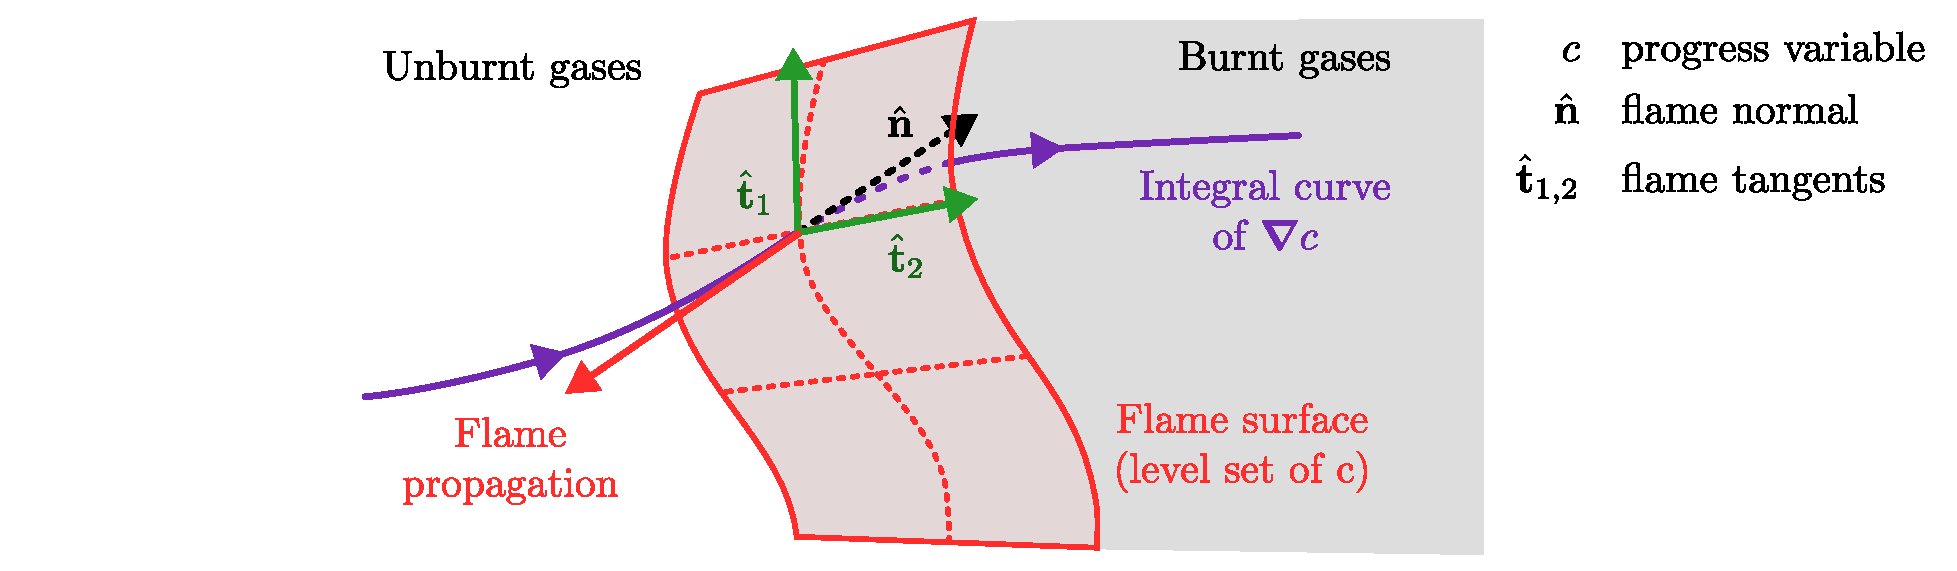
\includegraphics[scale=0.43]{assets/flamelet.pdf}
    \label{fig:flamelet}
    \caption{Diagram of the 3D flame surface model used below.}
\end{figure}

Defining the inverse thermal Peclet number: $\d = l_\rm{th} / L$ as the asymptotic parameter used by \cite{pelce1982InfluenceHydrodynamicsDiffusion,matalon1982FlamesGasdynamicDiscontinuities} to describe flame thickness alongside the Zeldovich number $\Ze$ which loosely prescribes reaction zone thickness relative to the flame thickness, the work of \cite{pelce1982InfluenceHydrodynamicsDiffusion,matalon1982FlamesGasdynamicDiscontinuities} primarily finds that the incompressible Navier-Stokes (NS) equations are suitable approximations of gas flow on either side of a premixed deflagration which is deficient in one reactant:
\begin{subequations}
\begin{boxaliat}{2}
\label{eqn:hydro-incomp} \vec{\nabla}\cdot\vec{u} &= 0                         &&+ \cl{O}\left( \d^2 \right), \\
\label{eqn:hydro-u} \r \mdv{\vec{u}}{t} &= - \vec{\nabla}p + \d\Pr \lap\vec{u} &&+ \cl{O}\left( \d^2 \right).
\end{boxaliat}
\end{subequations}
So these equations are valid on either side of the flame, which we describe mathematically by the level set of a function $F = 0$. The asymptotic papers make the additional assumption that this level set looks like the graph of a function in $y$, $f(y, t)$, such that e.g. in two-dimensions $F \equiv x - f(y, t)$. For numerical purposes, it is usually easiest to define this level set via the progress variable:
\begin{equation}
c \equiv \frac{Y_\a - Y_{\a, 1}}{\bbra{Y_\a}_V}
\end{equation}
for one of the species $\a$, so $F \equiv c - c^*$. The graph assumption is not the case for flames typically, so we instead rely on the level set formulation.

The \emph{product-pointing} normal (i.e. the normal which points towards the hot, light reaction products) is easily defined by:
\begin{equation}
\uvec{n} \equiv \frac{\vec{\nabla}c}{\norm{\vec{\nabla}c}} \bigg|_{F^-}.
\end{equation}
which is the unit normal vector pointing forward along the integral curve of $\vec{\nabla} c$ which goes through the relevant point at the flame surface. The reactant-pointing normal may also be used, which just results in a change in sign. We use the product-pointing normal so we start off without negatives. The absolute speed of the flame at a point on the flame is the component of the flame motion $\ndt{\vec{f}}$ which moves away from the products:
\begin{subequations}
\begin{equation}
S_a \equiv - \ndt{\vec{f}} \cdot \uvec{n},
\end{equation}
and the displacement speed also considers the effect of the fluid moving at the products, opposing flame motion:
\begin{equation}
S_d \equiv (\vec{u} - \ndt{\vec{f}}) \cdot \uvec{n} \,\big|_{F^-} = S_a + \vec{u} \cdot \uvec{n} \,\big|_{F^-}.
\end{equation}
Hence, considering the advection equation for the flame: $\partial c / \partial t + \ndt{\vec{f}}\cdot \vec{\nabla}c = 0$ we find the following simple expressions for absolute and displacement speed:
\begin{align}
S_a &= \frac{1}{\norm{\vec{\nabla}c}} \pdv{c}{t} \,\bigg|_{F^-} \\
S_d &= \frac{1}{\norm{\vec{\nabla}c}} \mdv{c}{t} \,\bigg|_{F^-}
\end{align}
In this context, the species conservation equation may be used:
\begin{align}
\r \mdv{c}{t} &= \frac{1}{\bbra{Y_\a}_V} \cdot \r \mdv{Y_\a}{t} = \frac{1}{\bbra{Y_\a}_V} \left( \ndt{\vr}_\a - \vec{\nabla} \cdot (\r \vec{V}_{\!\a} Y_\a) \right), \\
\implies \quad \Aboxed{ S_d &= \frac{1}{\r \norm{\vec{\nabla}c} \bbra{Y_\a}_V} \left[ \ndt{\vr}_\a - \vec{\nabla} \cdot (\r \vec{V}_{\!\a} Y_\a) \right] \bigg|_{F^-} . }
\end{align}
\end{subequations}

It was primarily the work of Markstein in his seminal papers \cite{markstein1951ExperimentalTheoreticalStudies,markstein1953InstabilityPhenomenaCombustion,markstein1964NonsteadyFlamePropagation} which brought forth the idea that changes in flame speed away from its \emph{unstretched} speed, the laminar flame speed, is proportional to the amount of stretching that the flame experiences. Although Markstein first suggested a simple relationship between flame speed and curvature, it is now accepted that, at least in the hydrodynamically unstable regime, a dependence with the full \emph{flame stretch} is required. The dimensional and non-dimensional forms of these relations for consumption and displacement speed therefore follow: 
\begin{subequations}
\begin{alignat}{4}
S_{c/d}   &= S_L &&+ l_\rm{th} \Mk_{c/d}&&( -\bb{K}   &&) \\
S_{c/d}^* &= 1   &&+        \d \Mk_{c/d}&&( -\bb{K}^* &&)
\end{alignat}
\end{subequations}
with $\bb{K}$ being the flame stretch as elaborated in \cite{matalon1982FlamesGasdynamicDiscontinuities,candel1990FlameStretchBalance,clavin1985DynamicBehaviorPremixed}. This flame stretch obeys the formula:
\begin{subequations}
\begin{align}
(-\bb{K}) &= S_a (\vec{\nabla}\cdot\uvec{n}) + \uvec{n} \cdot \vec{\nabla} \cross (\vec{u}\cross \vec{n}) \Big|_{F^-} \\
&= S_d (\vec{\nabla}\cdot\uvec{n}) + \left[ (\uvec{n}\otimes\uvec{n}) : \vec{\nabla}\vec{u} - \vec{\nabla} \cdot \vec{u} \right] \Big|_{F^-} \\
&= S_d (\vec{\nabla}\cdot\uvec{n}) + \left(\uvec{t}_1\otimes\uvec{t}_1 + \uvec{t}_2\otimes\uvec{t}_2\right) : \bb{E} \,\Big|_{F^-} \\
&= S_d \kappa + E
\end{align}
\end{subequations}
depending on the flame's displacement speed, curvature $\k$ and strain $E$:
\begin{subequations}
\begin{align}
\kappa &\equiv \vec{\nabla}\cdot\uvec{n}, \\
E &\equiv \left(\uvec{t}_1\otimes\uvec{t}_1 + \uvec{t}_2\otimes\uvec{t}_2\right) : \bb{E} \,\Big|_{F^-} = \left[ (\uvec{n}\otimes\uvec{n}) : \vec{\nabla}\vec{u} - \vec{\nabla} \cdot \vec{u}\right] \, \Big|_{F^-}, \\
\bb{E} &= \frac{1}{2}\left(\vec{\nabla}\vec{u} + (\vec{\nabla}\vec{u})^T\right)
\end{align}
where $\bb{E}$ is the strain rate tensor and the vectors $\uvec{n}$, $\uvec{t}_1$ and $\uvec{t}_2$ form a moving frame on the flame surface (assuming a three-dimensional system):
\begin{equation}
\uvec{t}_{1, 2} \cdot \uvec{n} = 0
\quad \text{and} \quad
\uvec{t}_{1} \cdot \uvec{t}_2 = 0.
\end{equation}
\end{subequations}
Finally, the values $\Mk_{c/d}$ are the \emph{Markstein numbers} for the consumption and displacement speed of the flame. Classic formulae used for these values are known as the \emph{Clavin-Williams formulae} \cite{clavin1982EffectsMolecularDiffusion}:
\begin{subequations}
\begin{alignat}{2}
\Mk_d &= \Mk_1 + && \frac{1}{2}\Ze (\Le - 1) \Mk_2, \\
\Mk_c &=         && \frac{1}{2}\Ze (\Le - 1) \Mk_2,
\end{alignat}
\end{subequations}
placeholder
\begin{subequations}
\begin{alignat}{2}
\Mk_1 &\equiv \frac{1 + q}{q} \ln (1 + q)             && > 0, \\
\Mk_2 &\equiv \int_{-\infty}^0 \ln (1 + q e^x) \dd{x} && > 0.
\end{alignat}
\end{subequations}


% jump conditions (use matalon independent flame equations)
% enhancement factors
% Local flame speeds etc.
% integral curves, contours and averaged vs summed local speeds




\section{Own Work}

\begin{figure}[t]
    \centering
    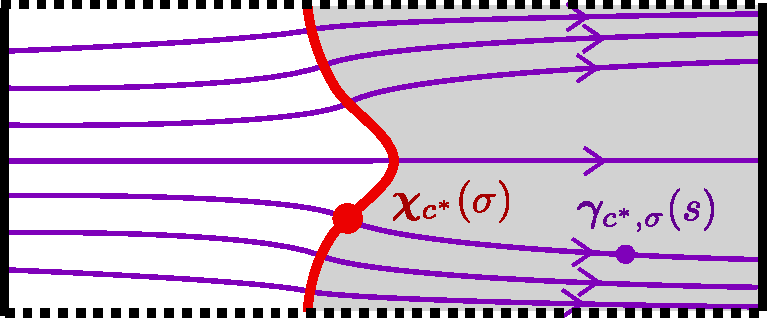
\includegraphics[scale=0.43]{assets/2d-flame-int-curves.pdf}
    \label{fig:int-curves}
    \caption{caption}
\end{figure}

These are sets depending on time, $t$, which we ignore below for brevity
\begin{subequations}
\begin{alignat}{2}
\chi_{c^*}       &\equiv \Big\{ \vec{\chi}_{c^*}(\sigma)  \, &&| \  c\big(\vec{\chi}_{c^*}(\sigma)\big) = c^* \Big\} \\
\g_{c^*, \a} &\equiv \Big\{ \vec{\g}_{c^*, \s}(s) \, &&| \  \vec{\g}_{c^*, \s}' =  \vec{\nabla}c / \norm{\vec{\nabla}c} \big|_{\vec{\g}_{c^*, \s}} \ \text{and} \  \vec{\g}_{c^*, \s}(0) = \vec{\chi}_{c^*}(\sigma) \Big\}
\end{alignat}
\end{subequations}
we find that the set integral curves does not change with time or the contour progress variable $c^*$ and covers domain:
\begin{subequations}
\begin{align}
A &= \big\{ \vec{\g}_{c_1, \s_1}(s_1) \, | \ s_1, \ \s_1 \ \text{and} \ \vec{\g}_{c_1, \s_1} \in \g_{c_1, \s_1} \big\} \\
&= \big\{ \vec{\g}_{c_2, \s_2}(s_2) \, | \ s_2, \ \s_2 \ \text{and} \  \vec{\g}_{c_2, \s_2} \in \g_{c_2, \s_2} \big\}
\end{align}
\end{subequations}
where $c_1 \neq c_2$. This ensures that integral quantities over the whole domain $A$ are exactly calculated by the continuous summation of integrals of the same quantity over each integral curve. For consumption speed $S_c$, this means that:
\begin{equation}
S_{c, \rm{loc}}(\s) = \frac{1}{\r_1 \bbra{T}_A} \int_{s_1}^{s_2} \frac{\ndt{\cl{T}}(\s, s)}{c_p(\s, s)} \dd{s},
\quad \text{and} \quad
\overline{S_{c, \rm{loc}}} = \frac{1}{L[\chi]} \int_{\s_1}^{\s_2} S_{c, \rm{loc}}(\s) \dd{\s}
\end{equation}
so
\begin{subequations}
\begin{align}
S_c &= \frac{1}{w \r_1 \bbra{T}_A} \int_A \frac{\ndt{\cl{T}}}{c_p} \dd{A} = \frac{1}{w \r_1 \bbra{T}_A} \int_{\s_1}^{\s_2} \int_{s_1}^{s_2} \frac{\ndt{\cl{T}}(\s, s)}{c_p(\s, s)} \dd{s} \dd{\s} \\
&= \frac{1}{w} \int_{\s_1}^{\s_2} S_{c, \rm{loc}}(\s) \dd{\s} = \frac{L[\chi]}{w} \cdot \overline{S_{c, \rm{loc}}}
\end{align}
\end{subequations}

% This means that integral quantities over the whole domain (S_c) can be exactly calculated through integrals over the curve of the same integral values (S_c,loc) over individual integral curves
% For S_c this turns out to be: integral over area = integral over x then y = integral over integral curve then contour

% Our contour finding algorithm is the marching squares algorithm which, as the name suggests, requires a cartisian grid of input data. We interpolate our unstructured mesh-free nodes onto a cartesian grid using cubic splines. Analyse only the DNS nodes which are in a rectangle around the flame so as to be non-negligible to same computational time. The contours may then be found for any progress variable c^*. The chemical progress variable c_Y was chosen here for the same reasons as Day et al and Howarth 2022 to better represent flame locations and reduce closed loop contours (C_Y = C_T FOR IDEALISED FLAMES, THEY HAVE NON-IDEALISED FLAMES). Note that the choice of the flame location is entirely arbitrary as a function of a continuous progress variable (in the asymptotic regime we essentially have discontinuous progress variable c = 0, the reactants, and c = 1, the products) so we are forced to make some sensible choice. we call this choice the flame progress variable c_flame, and take it to be a value of progress variable which best represents the location of highest heat release. Any other 'metric' could be used justifiably, and we hope at this stage that the value of the Markstein number is independent of this choice
% On this flame contour, normals may be calculated by travelling short distances along integral curves and used to calculate rate of strain and curvature. To calculate curvature we use a two point finite difference stencil:

% Rate of strain is calculated by the formula ( -- ) where spatial derivatives are easily calculated on the interpolated data via finite differences on the mesh points. Theoretically, rate of strain is evaluated just ahead of the flame, at f^-. In the context of simulation data this is again ambiguous as above, so we must choose its location. Normals are already treated to represent the shape of the flame, but for the upstream hydrodynamics, we must use some other metric. Hence, we choose to use a smaller progress variable, more representative of the reactant mixture location at the beginning of reaction, c_up. Rate of strain and all other evaluations of u will take place at the intersection of the c = c_up contour and the relevant integral curve. Note that we could instead evaluate values using a threshold density, but this is equivalent to using a temperature-based progress variable value.

% Flame thicknesses may be evaluated for each integral curve too. In Howarth and Aspden 2022 they have strong turbulence effects so the flame thickness vary significantly between integral curves. For these idealised laminar flames, however, we find that the flame thicknesses do not change significantly (1% or something?) so diffusive thicknesses are used unlike Howarth

% Displacement speed may be evaluated as in the previous section (equation 20f), but the evaluation of diffusive fluxes from the interpolated data generates spurious noise. Instead, we evaluate S_d from S_d = S_a + u . n. S_a may be simply estimated at steady states by assuming f dot is travelling horizontally, so then fdot = (u_in - S_c)e_x hat and ... 


% The mixing of u on upstream and n on flame contours may seem dubious, but actually when we do this our regression improves, justifying it quantitatively




% \chapter{Delay Boundary Conditions} \label{ch:delay-bcs}
% \section{Methodology}

\section{Implementation}

\begin{figure}[h]
\centering
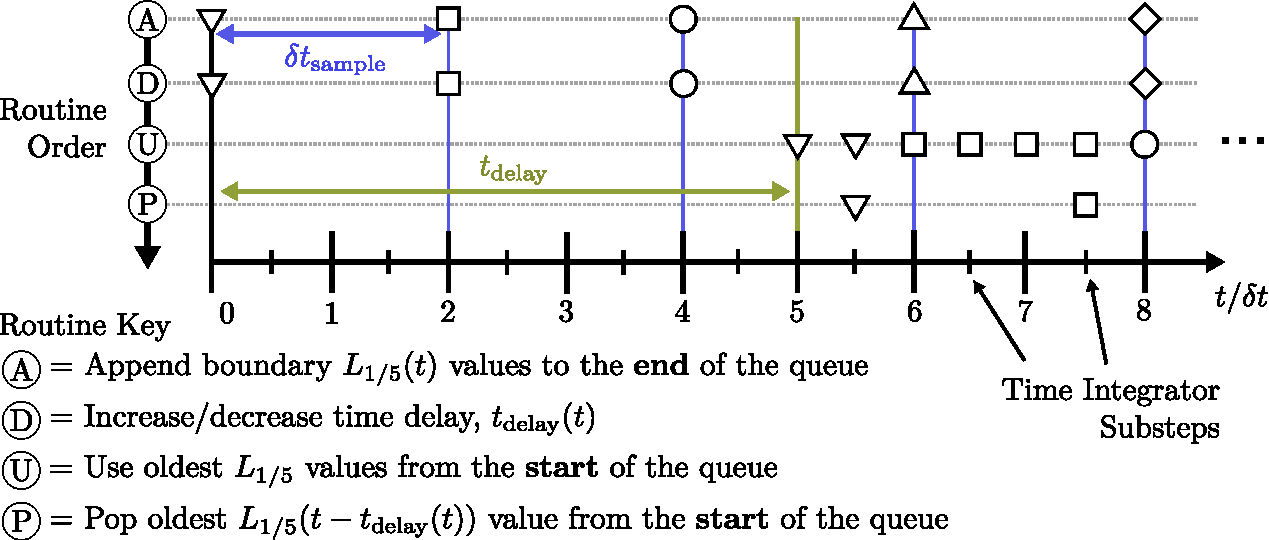
\includegraphics[scale=0.6]{assets/imgs/delay_bc_code_schematic.pdf}
\label{fig:schematic}
\caption{Schematic for delay BCs implemented into a multistage time integrator. }
\end{figure}


\begin{itemize}
\item Queues are filled with $L$ values as well as 
\end{itemize}

\subsection{Overcoming Instabilities}


\section{Results}





% \chapter{Conclusion} \label{ch:conc}
% CONCLUSIONS

% \chapter{Plan For Upcoming Years} \label{ch:plan}
% \section{Future Work}




\section{Planning}

\blue{Gantt Chart!!}


\printbibliography[title={References},heading=bibintoc]


\end{document}
